\documentclass[11pt, twoside, openany, a4paper]{book}

\usepackage{graphicx}
\ifx\pdfoutput\undefined
	% we are running LaTeX, not pdflatex
\else
	% we are running pdflatex, so convert .eps files to .pdf
	\usepackage{epstopdf}
\fi

\usepackage[usenames,dvipsnames]{pstricks}
\usepackage{auto-pst-pdf}
\usepackage[spanish,english]{babel}  % texto autogenerado en español o inglés
\usepackage[utf8]{inputenc} % Para linux, utf8

\setlength{\parskip}{0.3cm}


\begin{document}

\bibliographystyle{plain}
\nocite{*}
\selectlanguage{spanish}

\renewcommand{\tablename}{Tabla}
\renewcommand{\listtablename}{Índice de tablas}
\renewcommand{\bibname}{Bibliografía}

\pagestyle{empty}

\begin{titlepage} 
\begin{center} 
 
\includegraphics*[height=3.5cm]{images/logo_surcos.png} 

\vspace*{3.5cm} 
{\Huge \textbf{SURCOS: manual de usuario\\}}
\vspace*{1cm} 
{\normalsize Versión 6.0}\\
\vspace*{1cm} 
{\Large Javier Burguete$^1$, Asier Lacasta$^2$ y Pilar García-Navarro$^2$}\\ 
\vspace*{2.5cm} 
{\normalsize (1) Departamento de Suelo y Agua}\\
{Estación Experimental de Aula Dei / CSIC}\\ 
{Avda. Montañana 1005, 50059 Zaragoza, España}\\ 
\vspace*{1cm} 
{\normalsize (2) Área de Mecánica de Fluidos}\\ 
{Centro Politécnico Superior, Universidad de Zaragoza}\\
{María de Luna 3, 50018 Zaragoza, España}\\
\vspace*{1cm} 
{\normalsize \today}\\ 
\end{center} 
\end{titlepage} 
\cleardoublepage

\pagestyle{plain}
\pagenumbering{roman} % las primeras paginas las numeramos con numeros romanos

\tableofcontents
\listoffigures

\cleardoublepage

\pagestyle{headings}
\pagenumbering{arabic} % las primeras paginas las numeramos con numeros romanos

\chapter*{¡Atención!}

Para ejecutar el programa \emph{surcos} en sistema operativo Windows, deberá
iniciar la aplicación desde la subcarpeta \emph{win32/bin/winsurcos.exe}, en
versiones de 32 bits, o \emph{win64/bin/winsurcos.exe} en versiones de 64 bits.

\begin{itemize}
\item La representación de los números reales se hace, según el estándar
internacional, separando los decimales mediante el ``.'' decimal.
\item Las unidades de todas las variables utilizadas y representadas están en
Sistema Internacional.
\end{itemize}

El programa ha sido probado en los siguientes sistemas operativos de Microsoft:
\begin{itemize}
\item Windows 10 32 bits.
\item Windows 10 64 bits.
\end{itemize}

La activación del idioma se hace mediante la modificación de la configuración
regional del sistema operativo. La versión 5.6 de este programa tiene soporte
idiomático en inglés, español, francés e italiano. 

Se han reportado problemas en la ventana de representación gráfica debidos a
fallos de configuración de OpenGL en el driver de la tarjeta gráfica. Inténtese
en ese caso instalar el driver más actualizado de la tarjeta gráfica.

También se han reportado fallos guardando el fichero de la gráfica cuando el
sistema Windows se ejecuta dentro de una máquina virtual de VirtualBox. En este
caso el problema se corrige desactivando la aceleración gráfica en la
configuración de VirtualBox.

Windows 10 es marcas registradas de Microsoft.

\setcounter{page}{1}

\chapter{Instrucciones de instalación}

\section{Descarga}

El programa \emph{surcos} puede ser descargado libremente en:
\begin{itemize}
\item \textit{http://digital.csic.es/handle/10261/75830}
\end{itemize}
El código fuente más reciente puede descargarse libremente, con una licencia de
tipo BSD, en:
\begin{itemize}
\item \textit{https://github.com/jburguete/surcos}
\end{itemize}

\section{Instalación}

La instalación del programa \emph{surcos} consiste simplemente en descomprimirlo
en la carpeta deseada. No obstante, se recomienda que tanto la carpeta donde se
instala el programa como los nombres de los ficheros generados no contengan
espacios ni símbolos raros. Se han reportado casos en los que el podría no
encontrar los ficheros y no ejecutar la simulación.

\section{Ficheros del programa}

El programa consta de las siguientes carpetas:
\begin{description}
\item[win32/bin]
\item Carpeta que contiene el ejecutable, los ficheros ejecutables de las
librerías y los ficheros de diagramas en la versión para Windows de 32 bits.
\item[win32/etc]
\item[win32/lib]
\item Estas dos carpetas contienen algunos ficheros de las librerías para
Windows de 32 bits.
\item[win32/share]
\item Carpeta que contiene los ficheros de idiomas para Windows de 32 bits.
\item[win64/bin]
\item[win64/etc]
\item[win64/lib]
\item[win64/share]
\item Carpetas equivalentes a las anteriores para la versión de 64 bits.
\item[examples]
\item Carpeta que contiene ficheros de ejemplo.
\item[src]
\item Carpeta que contiene el código fuente del programa \emph{surcos} y el
código fuente de las librerías utilizadas.
\end{description}

\section{Compilación del código fuente}

El código fuente está escrito en lenguaje C y se han usado en su compilación
herramientas libres de GNU: gcc, gmake, aclocal, autoconf y pkg-config. La
versión para Windows se ha compilado además usando msys/mingw.

El programa \emph{surcos} hace uso de las siguientes librerías:
\begin{description}
\item[libiconv] (http://ftp.gnu.org/pub/gnu/libiconv)
\item[zlib] (http://sourceforge.net/projects/libpng)
\item[libxml] (http://xmlsoft.org)
\item[libffi] (ftp://sourceware.org/pub/libffi)
\item[glib] (http://ftp.gnome.org/pub/gnome/sources/glib)
\item[gettext] (http://ftp.gnu.org/pub/gnu/gettext)
\item[libpng] (http://sourceforge.net/projects/libpng)
\item[freetype] (http://sourceforge.net/projects/freetype)
\item[fontconfig] (http://fontconfig.freedesktop.org)
\item[pixman] (http://www.cairographics.org)
\item[cairo] (http://www.cairographics.org)
\item[atk] (http://ftp.gnome.org/pub/gnome/sources/atk)
\item[pango] (http://ftp.gnome.org/pub/gnome/sources/pango)
\item[gdk-pixbuf] (http://ftp.gnome.org/pub/gnome/sources/gdk-pixbuf)
\item[gtk+] (http://ftp.gnome.org/pub/gnome/sources/gtk+)
\item[freeglut] (http://sourceforge.net/projects/freeglut)
\item[jb] (https://github.com/jburguete/jb)
\end{description}

Una vez instaladas y configuradas todas estas herramientas y librerías la
secuencia para compilar el programa consiste en hacer en una terminal:
\begin{enumerate}
\item cd 5.6
\item ./build
\end{enumerate}
En algunos sistemas hay que hacer alguna corrección. Consúltese el inicio del
fichero README.md donde se dan instrucciones más detalladas en algunos sistemas.

El programa \emph{surcos} ha sido compilado y probado en los siguientes sistemas
operativos:
\begin{itemize}
\item Arch Linux
\item Debian Linux 12
\item Devuan Linux 4
\item DragonFly BSD 6.4
\item Fedora Linux 38
\item FreeBSD 13.2
\item Gentoo Linux
\item Linux Mint DE 5
\item MacOS Ventura + Homebrew
\item Manjaro Linux
\item Microsoft Windows 10 64 bits + MSYS2
\item NetBSD 9.3
\item OpenBSD 7.3
\item OpenIndiana Hipster
\item OpenSUSE Linux Leap 15.5
\item Ubuntu Linux 23.04
\end{itemize}

\cleardoublepage

\chapter{Ventanas de la aplicación}

En este capítulo se explicarán las ventanas de las que dispone el programa.

\section{Ventana Principal}

La ventana principal aparece al inicio del programa y es utilizada como interfaz básica de interactuación con el usuario. En ella se incluyen botones para acceder al resto de ventanas que en este capítulo se presentan.\\

\begin{figure}[!h]
\begin{center}
\includegraphics*[height=1.4cm]{images/mprincipal.png}
\caption{Ventana principal inicial de la aplicación \emph{surcos}}\label{mainWindow}
\end{center}
\end{figure}

\begin{table}[h]\footnotesize
\begin{center}
\begin{tabular}{llr}
\hline
\multicolumn{2}{c}{Elemento} \\
\cline{1-2}
Icono & Acción & Funcionalidad \\
\hline
Salir & Click & Salir de la aplicación\\
Abrir & Click & Abrir ventana de carga de caso \\
Configurar & Click & Abrir ventana de configuración de caso \\
Ejecutar & Click & Ejecutar caso \\
Gráficos & Click & Abrir ventana de visualización de resultados  \\
Sumario & Click & Abrir ventana de sumario \\
Ayuda & Click & Créditos \\
\hline
\end{tabular}
\end{center}
  \caption{Descripción de las diferentes acciones disponibles en el menú principal de la aplicación \emph{surcos}}\label{mainWindowIcons}
\end{table}

A través de los iconos de la tabla \ref{mainWindowIcons} podemos acceder a las diferentes funcionalidades del programa.\\
\section{Configuración de caso}
\subsection{Ventana Configuración de Geometría}

El programa \emph{surcos} simula riego en redes de surcos en tablares de forma cuadrilátera. En la ventana de configuración de geometría (ver figura \ref{geomWindow}), podemos modificar la topografía del problema modificando los cuatro vértices que definen el tablar.

\begin{figure}[!h]
\begin{center}
\includegraphics*[width=\textwidth]{images/confGeom.png}
\qquad
\caption{Ventana de configuración de geometría}\label{geomWindow}
\end{center}
\end{figure}

Como puede verse en la figura \ref{geomWindow}, el surco de distribución se localiza entre los puntos 1 y 2 y el surco de recirculación, si lo hubiera, entre los puntos 3 y 4. Los surcos de riego se localizan perpendicularmente a los anteriores.

\subsection{Ventana Configuración de surcos}

\begin{figure}[!h]
\begin{center}
\includegraphics*[width=\textwidth]{images/confSurco.png}
\qquad
\caption{Ventana de configuración de surcos}\label{confSurcos}
\end{center}
\end{figure}

En la ventana \ref{confSurcos} tenemos las propiedades de los surcos que vamos a simular desglosados en tres tipos: Distribución, recirculación y riego (siendo éste último el que define los surcos de riego propiamente). Estas opciones estarán activadas o desactivadas en función de que existan o no tanto surcos de riego como  surco de recirculación.

Las propiedades configurables para los surcos son las que se recogen en la figura \ref{confSurcos}.

\subsection{Ventana Configuración de entradas}

\begin{figure}[!h]
\begin{center}
\includegraphics*[width=\textwidth]{images/confInput.png}
\qquad
\caption{Ventana de configuración de las entradas}\label{input}
\end{center}
\end{figure}

En la ventana \ref{input} se configuran las entradas de agua y fertilizante. Cada entrada está definida por un punto del tablar, los tiempos inicial y final de la descarga, y un caudal constante. Este caudal es  volumétrico en el caso del agua y másico en el caso del fertilizante.

Es posible tratar hidrogramas más complejos definiendo varias entradas asociadas al mismo punto geométrico con el objeto de que se forme un hidrograma final como la suma de cada uno de ellos. 


\subsection{Ventana Configuración de fertilizante}

\begin{figure}[!h]
\begin{center}
\includegraphics*[width=\textwidth]{images/confFerti.png}
\qquad
\caption{Ventana de configuración de fertilizante}\label{ferti}
\end{center}
\end{figure}

La ventana \ref{ferti} sirve para definir la solubilidad del fertilizante. 

\subsection{Ventana Configuración de sondas}

\begin{figure}[!h]
\begin{center}
\includegraphics*[width=\textwidth]{images/confSondas.png}
\qquad
\caption{Ventana de configuración de sondas}\label{sondas}
\end{center}
\end{figure}

En la ventana \ref{sondas} se pueden definir el número de sondas que vamos a utilizar, así como las posiciones geométricas de las mismas. Nótese que si el punto cae fuera del surco, se aproximará la posición a la más cercana dentro del tablar. 

\subsection{Ventana Configuración de parámetros avanzados}

\begin{figure}[!h]
\begin{center}
\includegraphics*[width=\textwidth]{images/confParam.png}
\qquad
\caption{Ventana de configuración de parámetros avanzados}\label{param}
\end{center}
\end{figure}

En la ventana \ref{param} se recogen las opciones de configuración de la simulación. En ella, podemos modificar los valores relacionados con la simulación numérica.

\begin{description}
\item{Tiempo máximo de duración de la simulación}: Normalmente el programa \emph{surcos} simula hasta que todo el agua se ha infiltrado en el terreno. Para evitar simulaciones demasiado largas, este parámetro permite definir el tiempo máximo en segundos en el que se aborta la simulación, aunque quede agua sin infiltrar en el sistema.
\item{CFL}: Parámetro numérico adimensional proporcional al paso de tiempo utilizado por el método matemático de resolución. Deben usarse valores entre 0 y 1. Valores cercanos a 1 son óptimos. Valores muy bajos pueden ralentizar considerablemente la ejecución.
\item{Periodo de volcado de datos}: Intervalo de tiempo de simulación cada cuanto se vuelcan los resultados numéricos en ficheros.
\item{Número de celdas del canal de distribución (entre surcos)}: Número de celdas que contiene la malla en los canales de distribución y de recirculación entre cada 2 confluencias con los surcos de riego.
\item{Número de celdas de los surcos de riego}: Número de celdas que contiene la malla en cada surco de riego.
\end{description}

De ellos, es importante tener en cuenta que aparece la condición CFL relacionada con la estabilidad numérica del método y la cual es necesario que sea menor que 1 $(CFL < 1)$. Además aparece un valor para seleccionar en el número de celdas para los distintos surcos. Es necesario tener en cuenta que este valor está relacionado con la calidad de la solución pero también con la duración del cálculo. Otro de los valores es la periodicidad de los volcados, de tal forma que podremos obtener $ n=\frac{t_s}{p_v}$ instantaneas de evolución, siendo $ t_s $ el tiempo de simulación y $ p_v $ el periodo de volcado. 

Los números de celdas también son decisivos en la velocidad de cálculo de la simulación. Un número excesivamente grande ralentiza considerablemente la simulación mientras que con un número pequeño se pierde precisión. 

\section{Simulación}

La simulación del caso, previa configuración, se realizará mediante el botón ejecutar del menú principal:
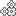
\includegraphics[height=0.4cm]{images/gtk-execute.png}

\section{Visualización de resultados}

%El programa puede mostrar tres tipos de resultados. El primero de ellos es modo textual y los otros dos son en modo gráfico

\subsection{Gráficas de resultados}

Las gráficas se controlan desde la ventana \ref{barraRepres}, donde se dispone de un dial para controlar el paso de tiempo representado en las variables que evolucionan con el tiempo. Además existe la posibilidad de seleccionar el surco, la variable o la sonda a representar. 

Se nos permite también guardar las gráficas pulsando en el botón que está al fondo del diálogo. En este case se guarda una imagen de la gráfica que hay en pantalla en un fichero en formato \emph{png}.

\begin{figure}[!h]
\begin{center}
\includegraphics*[width=\textwidth]{images/menuRepres.png}
\qquad
\caption{Ventana de selección de representación}\label{barraRepres}
\end{center}
\end{figure}

El programa \emph{Surcos} soporta tres tipos de representación. La primera de ellas es un mapa que representa de manera bidimensional la geometría de la red de surcos, posibilitando al usuario la representación de las variables descritas en la tabla \ref{tableVariablesMapa}.

\begin{table}[h]\footnotesize
\begin{center}
\begin{tabular}{ll}
\hline
Variable & Unidades \\
\hline
Calado & $m$ \\
Concentración de fertilizante & $ kg/m^3 $\\
Volumen de agua infiltrada por longitud de surco & $ m^2 $ \\
Masa de soluto por unidad de longitud & $ kg/m $ \\
\hline
\end{tabular}
\end{center}
  \caption{Variables visualizables en mapa de red de surcos}\label{tableVariablesMapa}
\end{table}

\begin{figure}[!h]
\begin{center}
\includegraphics*[width=\textwidth]{images/evo1.png}
\qquad
\caption{Ejemplo de representación en mapa de la variable calado}\label{evo1}
\end{center}
\end{figure}

Las otras dos son representaciones cartesianas de perfil longitudinal en los diferentes surcos y evoloución temporal en las diferentes sondas.

Las variables representables en el perfil longitudinal son las que aparecen en la tabla \ref{tableVariables2}.

\begin{table}[h]\footnotesize
\begin{center}
\begin{tabular}{ll}
\hline
Variable & Unidades\\
\hline
Calado & $m$ \\
Caudal & $ m^3/s $\\
Nivel (Cotas superficial y de fondo) & $ m $\\
Concentración de fertilizante & $ kg/m^3 $\\
Volumen de agua y masa de fertilizante superficial e infiltrados & $ m^2,\;kg/m $ \\
Tiempos de avance y receso & $ s $ \\
\hline
\end{tabular}
\end{center}
  \caption{Variables visualizables en cada surco}\label{tableVariables2}
\end{table}

\begin{figure}[!h]
\begin{center}
\includegraphics*[width=\textwidth]{images/evoSurco.png}
\qquad
\caption{Ejemplo de representación de un perfil longitudinal de las variables de volumen de agua y masa de fertilizante superficial e infiltrados en un surco}\label{evo2}
\end{center}
\end{figure}

Las variables representables en la evolución temporal son las que aparecen en la tabla \ref{tableVariables3}.

\begin{table}[h]\footnotesize
\begin{center}
\begin{tabular}{llr}
\hline
Variable & Unidades & Observaciones \\
\hline
Calado & $m$ \\
Concentración de fertilizante & $ kg/m^3 $\\
\hline
\end{tabular}
\end{center}
  \caption{Variables visualizables en cada sonda}\label{tableVariables3}
\end{table}

\begin{figure}[!h]
\begin{center}
\includegraphics*[width=\textwidth]{images/evoSonda.png}
\qquad
\caption{Ejemplo de representación de la evolución temporal de una sonda}\label{evo3}
\end{center}
\end{figure}

\subsection{Sumario}

El acceso al sumario se realiza mediante el botón 
\includegraphics[height=0.4cm]{images/gtk-edit.png}. Esta opción nos permite visualizar de manera textual tanto la configuración del riego como los resultados más relevantes de la simulación. Ambas opciones son las que aparecen en la figura \ref{wInforme}.

Entre los resultados se calculan las masas de agua y de fertilizante superficiales, infiltradas y percoladas, tanto en los surcos de riego como en los surcos de distribución. Se entiende como masa infiltrada la que penetra en el suelo y se queda en la zona de retención del suelo. La masa perdida por percolación no se considera por tanto como parte de la masa infiltrada.

El cálculo de la uniformidad de distribución se hace únicamente en los surcos de riego. La fórmula es la relación entre las medias infiltradas del 25\% de los puntos menos regados entre la media infiltrada total.

Finalmente, la eficiencia se calcula como la masa infiltrada en los surcos de riego dividida entre la masa total aplicada. Por lo tanto, tanto las masa percolada como la superficial o las infiltradas en los surcos de distribución y recirculación son consideradas como pérdidas en el cálculo de la eficiencia.

La ventana del sumario no permite guardar los resultados en un fichero. Para eso debe seleccionarse el texto a guardar con el ratón (o con el teclado), copiarse con las teclas \emph{Control+C} y pegarse en cualquier editor de texto como Microsoft Word.


\begin{figure}[!h]
\begin{center}
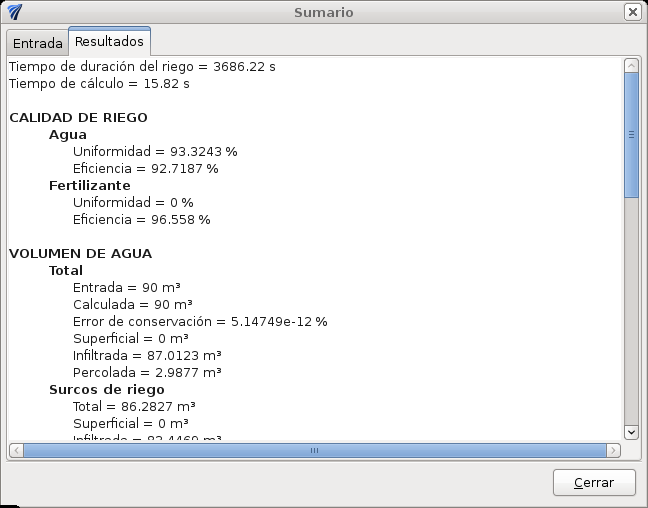
\includegraphics[width=0.45\textwidth]{images/sumario.png}
\qquad
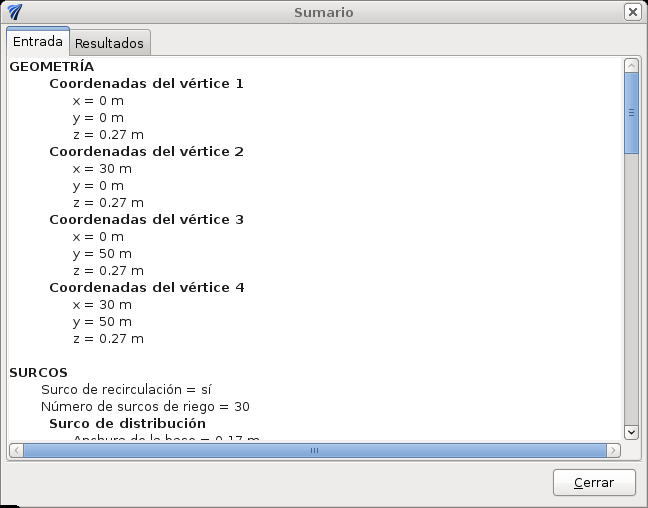
\includegraphics[width=0.45\textwidth]{images/sumario2.png}
\caption{Sumario de parámetros de entrada (Izquierda) y de resultados (Derecha)}\label{wInforme}
\end{center}
\end{figure}


%%%%%%%%%%%%%%%%%%%%%%%%%%%%%%%%%%%%%%%%%%%%%%%%%%%%%%%%%%%%%%%%%%%%%%%%%%%%%%%%%%%%%%%%%%%%%%%%%%%%%%%%5

\cleardoublepage

\chapter{Formato de los ficheros de entrada y salida}

En el programa \emph{Surcos}, los ficheros de entrada y de salida se almacenan
en una misma carpeta. El usuario puede elegir el nombre de esta carpeta,
pudiendo almacenar numerosos casos de estudio en distintas carpetas, pero los
ficheros de entrada y salida en cada carpeta tienen nombres fijos con una
nomenclatura que se detallará en las siguientes secciones. Todos estos ficheros
son ficheros de texto plano en formato ASCII.

\section{Ficheros de entrada}

\subsection{El fichero de geometría: field.in}

El fichero de geometría tiene el nombre:
\begin{itemize}
\item Carpeta\_del\_caso$\backslash$field.in
\end{itemize}

Este fichero está formado por el siguiente conjunto de números:\\
$o$ $n$ $s$\\
$x_1$ $y_1$ $z_1$\\
$x_2$ $y_2$ $z_2$\\
$x_3$ $y_3$ $z_3$\\
$x_4$ $y_4$ $z_4$\\
$b_b$ $z_b$ $H_b$ $D_b$ $R_b$ $\epsilon_b$ $r_b$ $K_b$ $a_b$ $i_b$ $d_b$
	$h_b$ $Q_b$ $c_b$\\
$b_i$ $z_i$ $H_i$ $D_i$ $R_i$ $\epsilon_i$ $r_i$ $K_i$ $a_i$ $i_i$ $d_i$
	$h_i$ $Q_i$ $c_i$\\
$b_c$ $z_c$ $H_c$ $D_c$ $R_c$ $\epsilon_c$ $r_c$ $K_c$ $a_c$ $i_c$ $d_c$
	$h_c$ $Q_c$ $c_c$\\
con:
\begin{description}
\item[$o$] 1 si hay surco de recirculación, 0 si no.
\item[$n$] Número de surcos de riego. Si sólo se quisiera simular un surco poner
	este número a 0 y se simulará sólo el surco de distribución.
\item[$s$] Solubilidad del fertilizante.
\item[$x_j$, $y_j$, $z_j$] Coordenadas del vértice $j$-ésimo que delimita la
	superficie del tablar.
\item[$b_k$] Anchura de la base del surco $k$.
\item[$z_k$] Pendiente de las paredes con respecto a la vertical del surco $k$.
\item[$H_k$] Profundidad del surco $k$.
\item[$D_k$] Distancia entre surcos del surco $k$.
\item[$R_k$] Capacidad de retención del suelo del surco $k$.
\item[$\epsilon_k$] Coeficiente de rozamiento aerodinámico de Burguete (si
	$\epsilon>0$) o modelo de fricción de Gauckler-Manning (si $\epsilon=0$)
	para el surco $k$.
\item[$r_k$] Número de Gauckler-Manning (si $\epsilon=0$) o longitud
	característica de rugosidad de Burguete (si $\epsilon>0$) del surco $k$.
\item[$K_k$] Coeficiente de infiltración de Kostiakov del surco $k$.
\item[$a_k$] Exponente de Kostiakov del surco $k$.
\item[$i_k$] Velocidad de infiltración saturada del surco $k$.
\item[$d_k$] Coeficiente de difusión del surco $k$.
\item[$h_k$] Profundidad inicial del agua del surco $k$.
\item[$Q_k$] Caudal inicial del surco $k$.
\item[$c_k$] Concentración inicial de fertilizante del surco $k$.
\end{description}
Los subíndices $k$ representan: $b$ para el surco de distribución, $i$ para
todos los surcos de irrigación (que por tanto tienen todos las mismas
características) y $c$ el surco de recirculación.

\subsection{Fichero de entradas de agua y fertilizante: input.in}

Las entradas de agua y fertilizante se definen en un fichero cuyo nombre es:
\begin{itemize}
\item Carpeta\_del\_caso$\backslash$input.in
\end{itemize}

Este fichero está formado por el siguiente conjunto de números:\\
$n_w$ $n_s$\\
$x_1$ $y_1$ $I_1$ $F_1$ $q_1$\\
$\cdots$\\
$x_{n_w}$ $y_{n_w}$ $I_{n_w}$ $F_{n_w}$ $q_{n_w}$\\
$x_1$ $y_1$ $I_1$ $F_1$ $q_1$\\
$\cdots$\\
$x_{n_s}$ $y_{n_s}$ $I_{n_s}$ $F_{n_s}$ $q_{n_s}$\\
con:
\begin{description}
\item[$n_w$, $n_s$] los números de entradas de agua y fertilizante
	respectivamente,
\item[$x_i$] coordenada $x$ del punto donde se produce la entrada $i$-ésima,
\item[$y_i$] coordenada $y$ del punto donde se produce la entrada $i$-ésima,
\item[$I_i$] tiempo inicial en el que se produce la entrada $i$-ésima,
\item[$F_i$] tiempo final en el que se produce la entrada $i$-ésima,
\item[$q_i$] caudal de la entrada $i$-ésima, en $m^3/s$ si la entrada es de
	agua y en $kg/s$ para las entradas de fertilizante.
\end{description}
Nótese que primero deben especificarse las $n_w$ entradas de agua y luego las
$n_s$ entradas de fertilizante.

\subsection{Fichero de tiempos de simulación: times.in\label{SecTiempos}}

Los tiempos característicos de simulación deben definirse en el fichero:
\begin{itemize}
\item Carpeta\_del\_caso$\backslash$times.in
\end{itemize}

Este fichero está compuesto por el siguiente conjunto de números:\\
$t_f$ $cfl$ $t_m$\\
donde:
\begin{description}
\item[$t_f$] es el tiempo total de simulación,
\item[$cfl$] es el número CFL que controla el tamaño de paso temporal,
\item[$t_m$] es el intervalo de tiempo cada cuanto se vuelcan los resultados en
	un fichero.
\end{description}

\subsection{Fichero de malla: mesh.in}

El número de celdas de la malla se especifica en el fichero:
\begin{itemize}
\item Carpeta\_del\_caso$\backslash$mesh.in
\end{itemize}

Este fichero está compuesto por los números:\\
$n_d$ $n_i$\\
con:
\begin{description}
\item[$n_d$] número de celdas de los surcos de distribución o de recirculación
	entre cada 2 surcos de riego,
\item[$n_i$] número de celdas en cada surco de riego.
\end{description}

\subsection{Fichero de sondas: probe.in}

Las sondas de medida pueden especificarse en el fichero:
\begin{itemize}
\item Carpeta\_del\_caso$\backslash$probe.in
\end{itemize}

Este fichero está formado por el siguiente conjunto de números:\\
$n_p$\\
$x_1$ $y_1$\\
$\cdots$\\
$x_{n_p}$ $y_{n_p}$\\
con:
\begin{description}
\item[$n_p$] número de sondas,
\item[$x_i$] coordenada $x$ del punto de la sonda $i$-ésima,
\item[$y_i$] coordenada $y$ del punto de la sonda $i$-ésima.
\end{description}

\subsection{Fichero de modelo: model.in}

Los modelos utilizados se definen en el fichero:
\begin{itemize}
\item Carpeta\_del\_caso$\backslash$model.in
\end{itemize}

Este fichero está formado por los números:\\
$m_f$ $m_i$ $m_u$ $m_a$\\
con:
\begin{description}
\item[$m_f$] 1 si hay fertilizante, 0 si no.
\item[$m_i$] 1 si hay infiltración, 0 si no.
\item[$m_u$] 1 si hay difusión subterránea, 0 si no.
\item[$m_a$] 1 si se usa el modelo de convección de Boussinesq, 0 si usa el
	modelo simple.
\end{description}

\section{Ficheros de resultados}

En el programa \emph{Surcos} los ficheros de resultados están codificados con
los siguientes nombres:
\begin{description}
\item[00b] Surco de distribución.
\item[00c] Surco de recirculación.
\item[xxx] Surco de riego, con $xxx$ representando el número de surco con 3
	dígitos. La numeración de estos surcos va de 0 a $n$-1 con $n$ el
	número total de surcos de riego.
\end{description}

Los ficheros de resultados son escritos en la misma carpeta donde se
encuentran los ficheros de entrada de datos. El programa genera 3 tipos
diferentes de ficheros de resultados, todos ellos en formato ASCII. 

\subsection{Ficheros de perfil longitudinal (xxx-yyy.out)}

El programa \emph{Surcos} genera un fichero donde se almacena el perfil
longitudinal de cada variable para cada surco y para cada paso de tiempo
definido en el intervalo de tiempo de volcado (véase la
sección~\ref{SecTiempos}).

El nombre de estos ficheros es de forma:
\begin{itemize}
\item $xxx-yyy.out$
\end{itemize}
donde $xxx$ representa el nombre del surco con la codificación descrita
anteriormente y $yyy$ representa el número de paso temporal en el que se
volcaron los resultados, especificado con 3 dígitos.

Estos perfiles son ficheros de 12 columnas de la forma:\\
\begin{tabular}{cccccccccccc}
$x_1$& $h_1$& $A_1$& $Q_1$& ${z_s}_1$& ${z_f}_1$& $-{A_i}_1$& $c_1$&
	$-{A_{ci}}_1$& $-{A_p}_1$& $-{A_{cp}}_1$& $\beta_1$\\
&&&&&&$\cdots$\\
$x_n$& $h_n$& $A_n$& $Q_n$& ${z_s}_n$& ${z_f}_n$& $-{A_i}_n$& $c_n$&
	$-{A_{ci}}_n$& $-{A_p}_n$& $-{A_{cp}}_n$& $\beta_n$
\end{tabular}\\\\
con:
\begin{description}
\item[$x_i$] la coordenada longitudinual del punto $i$-ésimo de la malla,
\item[$h_i$] el calado superficial del punto $i$-ésimo de la malla,
\item[$A_i$] el área transversal mojada superficial del punto $i$-ésimo de la
	malla,
\item[$Q_i$] el caudal superficial del punto $i$-ésimo de la malla,
\item[${z_s}_i$] la cota de la superficie del agua del punto $i$-ésimo de la
	malla,
\item[${z_f}_i$] la cota del fondo del punto $i$-ésimo de la malla,
\item[$-{A_i}_i$] la masa de agua infiltrada (negativa) por unidiad de longitud
	de surco del punto $i$-ésimo de la malla,
\item[$c_i$] la concentración superficial de fertilizante del punto $i$-ésimo de
	la malla,
\item[$-{A_{ci}}_i$] la masa de fertilizante infiltrada por unidad de longitud
	de surco (negativa) del punto $i$-ésimo de la malla,
\item[$-{A_p}_i$] la masa de agua percolada por unidad de longitud de surco del
	punto $i$-ésimo de la malla,
\item[$-{A_{cp}}_i$] la masa de fertilizante percolada por unidad de longitud
	de surco del punto $i$-ésimo de la malla,
\item[$\beta_i$] el coeficiente de convección de Boussinesq del punto $i$-ésimo
	de la mallar,
\item[$n$] el número de puntos de la malla que contiene el surco.
\end{description}

\subsection{Ficheros de tiempos de avance y receso (xxx.out)}

El programa \emph{Surcos} genera ficheros con los tiempos de avance y receso que
se producen para cada surco. El nombre de estos ficheros es de forma:
\begin{itemize}
\item $xxx.out$
\end{itemize}
donde $xxx$ representa el nombre del surco con la codificación descrita
anteriormente.

Estos ficheros son de 3 columnas de la forma:\\
\begin{tabular}{ccc}
$x_1$& ${t_a}_1$& ${t_r}_1$\\
&$\cdots$\\
$x_n$& ${t_a}_n$& ${t_r}_n$\\
\end{tabular}\\\\
con:
\begin{description}
\item[$x_i$] la coordenada longitudinual del punto $i$-ésimo de la malla,
\item[${t_a}_i$] el tiempo de avance del punto $i$-ésimo de la malla,
\item[${t_r}_i$] el tiempo de receso del punto $i$-ésimo de la malla,
\item[$n$] el número de puntos de la malla que contiene el surco.
\end{description}

\subsection{Ficheros de sondas (probes.out)}

El fichero donde se almacenan los resultados de las sondas tiene el nombre
\emph{probes.out}. Este fichero tiene el formato:\\
\begin{tabular}{cccccc}
$t_0$ & $h_{1,0}$ & $c_{1,0}$ & $\cdots$ & $h_{n_p,0}$ & $c_{n_p,0}$\\
&&&$\vdots$\\
$t_{n_t}$ & $h_{1,n_t}$ & $c_{1,n_t}$ & $\cdots$ & $h_{n_p,n_t}$ & $c_{n_p,n_t}$
\end{tabular}\\\\
con:
\begin{description}
\item[$t_j$] el tiempo $j$-ésimo, con 0 el instante inicial,
\item[$h_{i,j}$] el calado medido en la sonda $i$-ésima y en el tiempo
	$j$-ésimo,
\item[$c_{i,j}$] la concentración superficial de fertilizante medida en la sonda
	$i$-ésima y en el tiempo $j$-ésimo,
\item[$n_p$] el número de sondas,
\item[$n_t$] el número de pasos de tiempo.
\end{description}

\cleardoublepage

%\bibliography{bib/references}
%\cleardoublepage

\end{document}
